%!TEX root = ../Master_template.tex
\chapter{Related Work}



This chapter comprehensively summarizes the latest data augmentation methodologies designed for time series analysis. Time series tasks span a variety of domains; however, this work primarily focuses on two: \textbf{Time Series Forecasting (TSF)} and \textbf{Time Series Classification (TSC)}. Augmentation methods for forecasting are commonly categorized into four types: transformation-based, frequency-based, decomposition-based, and other approaches (refer to Section~\ref{sec: tsf_related}). For classification, augmentation methods are typically grouped into transformation-based, pattern-based, generative model-based, and decomposition-based categories (see Section~\ref{sec: tsc_related}).


Each category is discussed in detail, with formal definitions, mathematical formulations, pseudocode, and illustrative figures provided, where appropriate, to facilitate a deeper understanding of the augmentation methods. All mathematical representations in this chapter align with the formalism established in Section~\ref{section:formulation}.




\section{Time Series Forecasting } \label{sec: tsf_related}

\subsection{Transformation-based Augmentations} \label{section:transformation}


Transformation-based techniques include Gaussian noise injection~\cite{wen2019timeseriesanomalydetection}, window cropping~\cite{cui2016multiscaleconvolutionalneuralnetworks, Wen_2021}, window warping, and other methods~\cite{Wen_2021}. Initially developed in Computer Vision (CV), these methods have been adapted for time series analysis, specifically for tasks like time series classification and anomaly detection, showing significant effectiveness. These methods and more of them for the classification are detailed in Section~\ref{section:transformation2}. Nevertheless, the direct application of these augmentation techniques to TSF tasks generally does not produce significant advantages, as indicated by recent studies. The main factors contributing to the limited success in forecasting contexts are disturbances to the temporal order, such as introducing random noise or shifting the time series, or a lack of diversity in the generated augmented samples. These issues underscore the essential significance of preserving both diversity and coherence in augmentation methodologies tailored explicitly for forecasting tasks~\cite{Wen_2021, chen2023fraugfrequencydomainaugmentation, zhang2023diversecoherentaugmentationtimeseries, zhao2024dominantshufflesimplepowerful}. 



These traditional transformation-based augmentation methods were evaluated in the paper~\cite{chen2023fraugfrequencydomainaugmentation}, and the results indicate that they generally fail to improve performance over models trained without augmentation. Table~\ref{tab:Trad} reports the Mean Squared Error (MSE) for various models on the ETTh1 dataset with a prediction length of 96. As shown, most of these techniques—such as masking, flipping, and warping—tend to degrade performance and introduce distortions to the temporal structure. Other studies have similarly concluded that such transformations offer little to no benefit and distort the temporal dynamics of the time series signals, ultimately worsening model performance~\cite{Wen_2021, zhang2023diversecoherentaugmentationtimeseries, zhao2024dominantshufflesimplepowerful}.


\begin{table*}[h]
\centering

\begin{adjustbox}{max width=\textwidth}

\begin{tabular}{c|c|c|c|c|c|c|c}
\toprule
Method & Origin & Noise & Noise* & Mask-Rand. & Mask-Seg. &Flipping &Warping\\ \midrule
DLinear & 0.373 & 0.444 & \textbf{0.371} & 0.803 &0.448 & 0.544 &0.401  \\
FEDformer & \textbf{0.374} & 0.380 & 0.397 & 0.448 &0.433 & 0.420 &0.385  \\
Autoformer & \textbf{0.449} & 0.460 & 0.476& 0.608 & 0.568  & 0.446 &0.465  \\
Informer & 0.931 & 0.936 & 1.112 & \textbf{0.846} & 1.013 & 0.955 &1.265 \\\bottomrule
\end{tabular}
\end{adjustbox}
\vspace{-0.1cm}
\caption{MSE of various transformation-based data augmentation methods on the ETTh1 dataset with a prediction length of 96, as reported in~\cite{chen2023fraugfrequencydomainaugmentation}. “Origin” refers to training without augmentation. Across all four forecasting models, transformation-based augmentation methods tend to worsen performance.}
\label{tab:Trad}
\vspace{-0.3cm}
\end{table*}



\subsection{Frequency-based Augmentations}


Frequency-based methods, including time-frequency approaches, achieved significant popularity, resulting in the design and implementation of various techniques. These methods apply diverse augmentation strategies, including frequency masking, frequency mixing, perturbation of phase or magnitude of frequencies, shuffling of frequency components, and alteration of frequency components~\cite{chen2023fraugfrequencydomainaugmentation, zhao2024dominantshufflesimplepowerful, gao2021robusttadrobusttimeseries, freqpool, freqadd, arabi2024wavemaskmixexploringwaveletbasedaugmentations}. 


One of the foundational approaches in frequency-domain augmentation is RobustTAD~\cite{gao2021robusttadrobusttimeseries}, which applies perturbations to either the magnitude or phase of the frequency spectrum. Specifically, this method first obtains the frequency spectrum $F(\omega_k)$ of an input time series $x_t$ through the discrete Fourier transform (DFT):

\[ F(\omega_k) = \frac{1}{N}\sum_{t=0}^{N-1} x_t e^{-j2\pi kt/N}, \quad k=0,1,\dots,N-1,  \]


This spectrum can be decomposed into real and imaginary parts, represented as:

\[ F(\omega_k) = \Re[F(\omega_k)] + j\Im[F(\omega_k)], \]
where $\Re[F(\omega_k)]$ and $\Im[F(\omega_k)]$ are the real and imaginary parts of the spectrum respectively.

The amplitude spectrum $A(\omega_k)$ and phase spectrum $\theta(\omega_k)$  are derived as follows:

\[  A(\omega_k) = |F(\omega_k)| = \sqrt{\Re^2[F(\omega_k)] + \Im^2[F(\omega_k)]},  \]

and

\[ \theta(\omega_k) = \arctan\left(\frac{\Im[F(\omega_k)]}{\Re[F(\omega_k)]}\right) \]



To perform augmentation, RobustTAD selects segments of the frequency spectrum to modify. The length $K$ of each selected segment is determined proportionally by a hyperparameter ratio $r$: $K = r N'$ where $N'$ denotes the length of the spectrum~\cite{gao2021robusttadrobusttimeseries}.

For amplitude-based augmentation, the original amplitudes in the chosen segments are changed to values from a Gaussian distribution, which is controlled by a parameter for perturbation intensity. In the case of phase augmentation, the phase values within the selected segments are increased slightly by introducing controlled perturbations~\cite{gao2021robusttadrobusttimeseries}. While the original paper conducted experiments on anomaly detection, the studies~\cite{chen2023fraugfrequencydomainaugmentation, zhang2023diversecoherentaugmentationtimeseries, zhao2024dominantshufflesimplepowerful} have explored magnitude perturbation of RobustTAD for the multivariate TSF tasks. Phase perturbation has also been incorporated into RobustTAD for our experimentations.




Frequency Masking (FreqMask) and Frequency Mixing (FreqMix) are recent research studies on data augmentation for TSF that work on the frequency domain. They are straightforward but effective augmentation methods described in Figure~\ref{fig:freqmask}. FreqMask masks the signal's frequency components, eliminating specific events from the underlying system. On the other hand, FreqMix mixes frequencies from two randomly chosen series within the same batch, which exchange events between systems. To extract the frequency components for both methods, they rely on the fast Fourier transform (FFT)~\cite{chen2023fraugfrequencydomainaugmentation}. The complete pseudocode for these methods is available in Appendix~\ref{app:freqmask}.



\begin{figure}[h!]
    \centering
    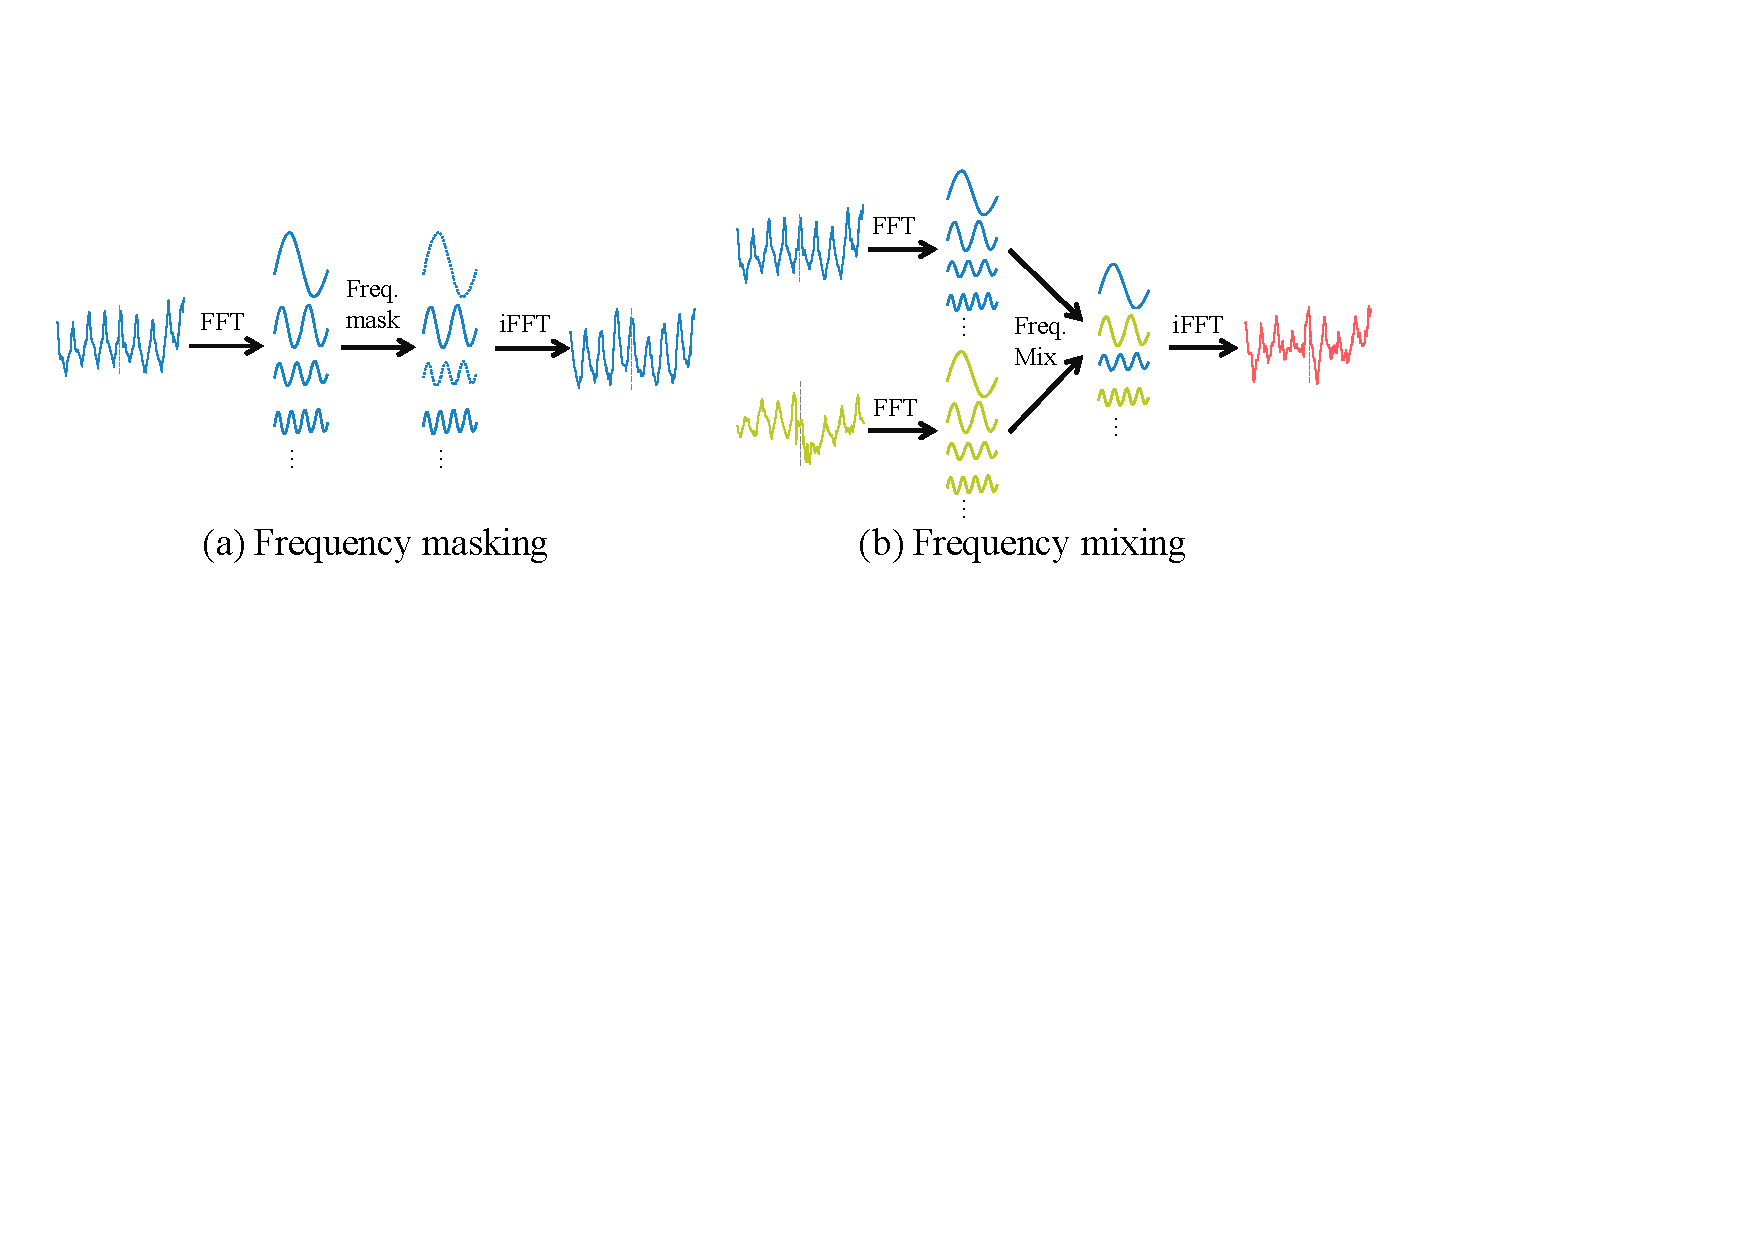
\includegraphics[page=1, width=0.9\textwidth]{./images/freqmaskmix.pdf}
\caption{Illustration of Frequency Masking and Frequency Mixing techniques. Both methods operate in the frequency domain by first applying a fast Fourier transform (FFT). Frequency Masking removes selected frequency components to suppress specific temporal patterns, while Frequency Mixing blends the frequency spectra of two series within the same batch to exchange dynamic characteristics~\cite{chen2023fraugfrequencydomainaugmentation}.}

    \label{fig:freqmask}
\end{figure}



% write about wavelet mask/mix add pictures only showing wavemask improvement. write description and the code.


Wavelet masking (WaveMask) and wavelet mixing (WaveMix) were introduced by~\cite{arabi2024wavemaskmixexploringwaveletbasedaugmentations} to address the limitations of FreqMask and FreqMix, which do not take the time domain into account. They are implemented the same way as FreqMask and FreqMix, but they apply the discrete wavelet transform (DWT) instead of the Fourier transform. Figure~\ref{fig:wavemask} illustrates the time-frequency analysis of the signal, and it shows the effectiveness of using wavelet transform to deliver frequency component information over time through different variable windows. WaveMask and WaveMix have been shown to outperform FreqMask and FreqMix methods on a small subset of datasets, indicating their potential for improved performance in TSF tasks~\cite{arabi2024wavemaskmixexploringwaveletbasedaugmentations}.






\begin{figure}[h!]
    \centering
    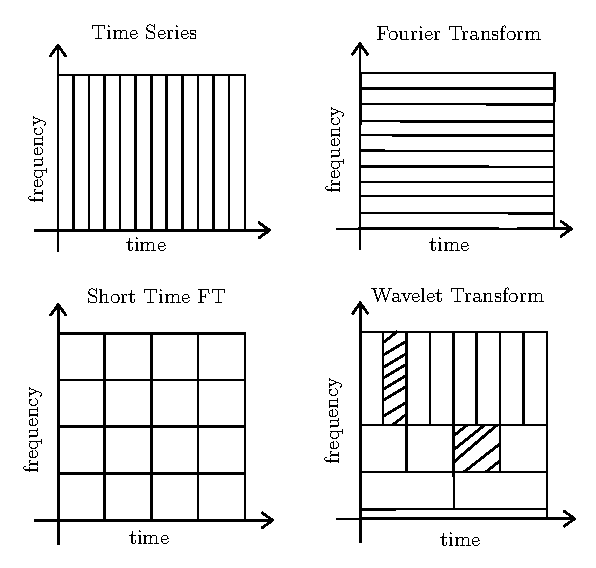
\includegraphics[page=1, width=0.6\textwidth]{./images/wavemask.pdf}
\caption{Time-frequency analysis methods, where the wavelet-based approach demonstrates how it captures localized frequency components using variable-sized windows~\cite{en16020764, arabi2024wavemaskmixexploringwaveletbasedaugmentations}.}
    \label{fig:wavemask}
\end{figure}


%write dominant shuffle and also say that they did not compare with WaveMask. add picture if there is peseduocode add it.




The paper by \cite{zhao2024dominantshufflesimplepowerful}  has mentioned that existing augmentations such as FreqMask and FreqMix may perturb the frequency components arbitrarily, which leads to significant deviations from the original time series data and introduce out-of-distribution (OOD) issues. The authors validate it through t-distributed stochastic neighbor embedding (t-SNE) visualizations. They have also proposed a new simple augmentation method named Dominant Shuffle and have conducted a comprehensive comparison with existing augmentation techniques. Dominant Shuffle obtains frequency components with the FFT and permutes randomly top $k$  dominant frequency components before reconstructing the augmented series. Figure~\ref{fig:domshuffle} depicts Dominant Shuffle augmentation, which changes the order of the three dominant frequency components. Their experimentations also include shuffling of not only dominant but also minor frequencies in the ablation study~\cite{zhao2024dominantshufflesimplepowerful}. 









\begin{figure}[h!]
    \centering
    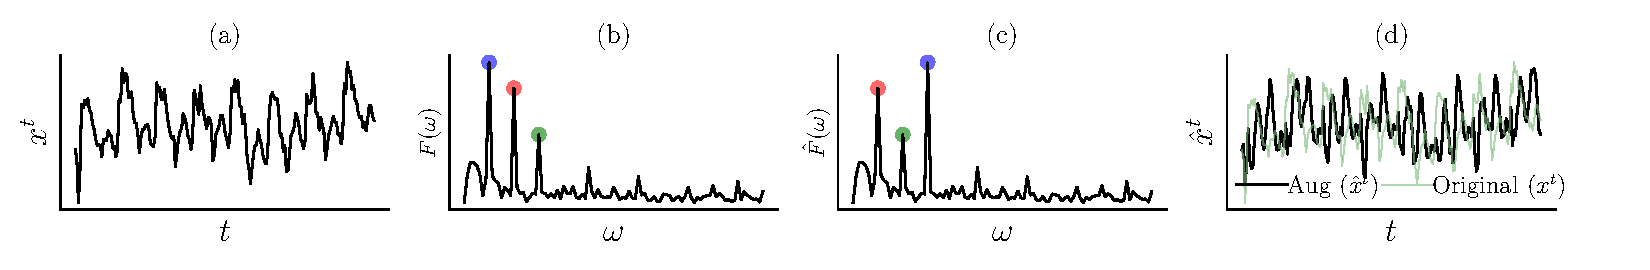
\includegraphics[page=1, width=0.9\textwidth]{./images/domshuffle.pdf}
    \caption{Illustration of the Dominant Shuffle augmentation technique, which permutes the top three dominant frequency components identified via FFT before reconstructing the time series~\cite{zhao2024dominantshufflesimplepowerful}.}
    \label{fig:domshuffle}
\end{figure}


%write freqadd, freqpool explain much possible you can. maybe two small paragprahs.

Other frequency-based augmentation techniques are FreqAdd~\cite{freqadd} and FreqPool~\cite{freqpool}, where the former modifies the frequency component and the latter compresses the frequency spectrum. FreqAdd chooses a low-frequency component after obtaining frequency components with FFT and sets its magnitude to half of the maximum magnitude in the corresponding channel. Experimental results demonstrate that FreqAdd reaches peak performance when it modifies a single, low-frequency component, whereas low-frequency components pertain to the lower-frequency spectrum segment and contain slower fluctuations. On the other hand, FreqPool compresses the frequency spectrum by applying max-pooling along the frequency axis, which diminishes spectral resolution yet retains dominant frequency information~\cite{freqadd, freqpool}. \cite{zhao2024dominantshufflesimplepowerful} conducted a comprehensive evaluation of these augmentation strategies, validating their effectiveness, especially in multivariate TSF contexts.



\subsection{Decomposition-based Augmentations} \label{section:decom}







Decomposition-based methods primarily apply techniques such as Seasonal and Trend decomposition using Loess (STL)~\cite{cleveland1990stl} or Empirical Mode Decomposition (EMD)~\cite{huang1998empirical}. Early approaches applies EMD to decompose time series into Intrinsic Mode Functions (IMFs), which represent frequency components ranging from high-frequency oscillations to low-frequency variations. The residual is incorporated with each occurrence of an IMF, serving as a data augmentation method that filters out high-frequency noise~\cite{nam2020data}. Nonetheless, the drawback of this technique is that it fails to incorporate the time domain~\cite{zhang2023diversecoherentaugmentationtimeseries}. 

The recent augmentation method, Spectral and Time Augmentation (STAug), proposed by \cite{zhang2023diversecoherentaugmentationtimeseries}, relies on frequency and time domains. Figure~\ref{fig:staug} illustrates the methodology of STAug. It selects two time-series sequences randomly and decomposes both into multiple IMFs by utilizing EMD. After assigning weights from a uniform distribution for these decomposed components, they are recombined in a time-domain signal through a Mixup strategy~\cite{zhang2018mixupempiricalriskminimization} with a parameter $\lambda$ sampled from a Beta distribution. This step adds diversity by combining elements from various sequences in the time domain, using both temporal coherence and spectral attributes. The experimental results of the paper validated that STAug outperforms existing augmentation techniques across various benchmark datasets, including RobustTAD and TimeGAN~\cite{zhang2023diversecoherentaugmentationtimeseries}.




\begin{figure}[h!]
    \centering
    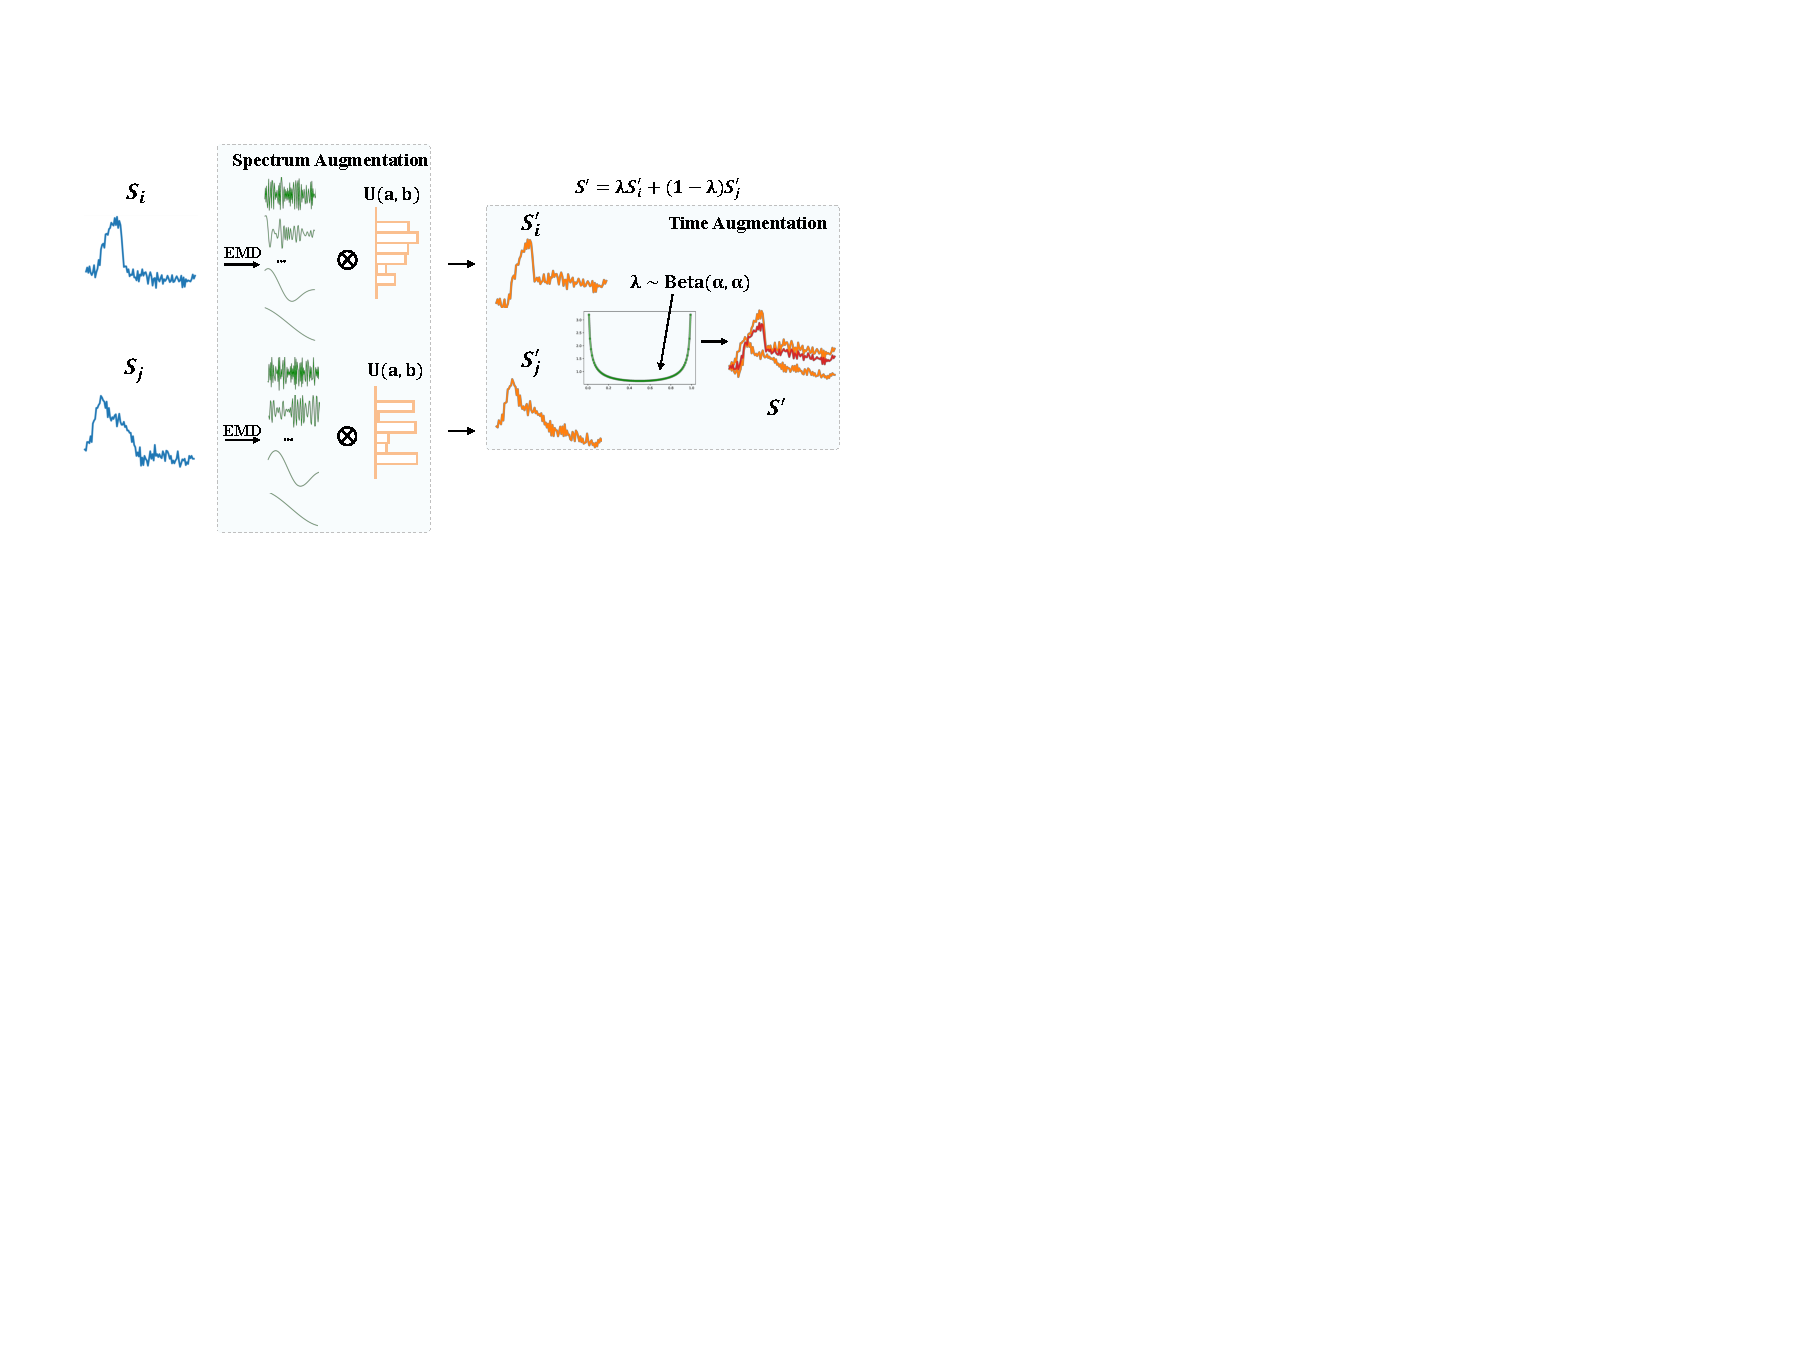
\includegraphics[page=1, width=0.9\textwidth]{./images/staug.pdf}
    \caption{STAug: A decomposition-based augmentation method that applies Empirical Mode Decomposition (EMD) and recombines IMFs using a Mixup strategy in the time domain~\cite{zhang2023diversecoherentaugmentationtimeseries}.}
    \label{fig:staug}
\end{figure}



\subsection{Other Approaches} \label{section:other}

This section presents various augmentation techniques grouped under \emph{other approaches}, including Moving Block Bootstrapping~\cite{mbb}, weighted Dynamic Time Warping Barycentric Averaging~\cite{asd}, Upsampling~\cite{upsample}, and generative model-based augmentations (e.g., TimeGAN~\cite{timegan}). These methods are categorized separately because they do not decompose time series nor explicitly function within frequency domains, amplitude spectra, or wavelet domains, in contrast to the previously reviewed techniques~\cite{asd, mbb, upsample, timegan}. 

The Upsample augmentation technique selects consecutive segments from the original time series, and a hyperparameter ratio $r$ determines the length of this segment. This segment is expanded to the original length of time series $T$ through linear interpolation, which helps to highlight data areas that forecasting models may overlook. As expressed by the authors, this technique operates as a ”magnifying glass”, enabling forecasting models to focus on local structures and intricate temporal patterns. The Upsample method has been evaluated against various augmentation methods, including fundamental and advanced techniques, primarily within univariate forecasting tasks. Empirical evidence shows that Upsample consistently surpasses alternative methods in predictive accuracy~\cite{upsample}. The method is assessed in multivariate forecasting contexts, where it exhibited successful results in the paper~\cite{zhao2024dominantshufflesimplepowerful}. Considering these documented results, the Upsample technique is incorporated into the empirical evaluations performed in this thesis study. 




% ASD

Different augmentation techniques using Dynamic Time Warping (DTW) to calculate pair-wise distances of training samples exist, and one of them is Dynamic Time Warping Barycentric Averaging (DBA), which generates augmented samples by averaging time series sets. There is another version called weighted DBA (wDBA), which assigns weights through the contribution of each time series toward the final one. \cite{asd} have proposed three versions of these augmentations based on the weighting: Average All (AA), Average Selected (AS), and Average Selected with Distance (ASD). wDBA with ASD is considered augmentation in our experimentation protocol and evaluated against other augmentation methods in earlier and recent papers for TSF. Specifically, after calculating the distances with DTW, wDBA applies an exponentially weighted sum to each sample’s top 5 closest neighbors to generate an augmented sample. This method is computationally expensive compared to the other methods in the experimentation. In the literature, this method is referred to interchangeably as ASD or wDBA; in this thesis, we consistently refer to it as wDBA~\cite{asd, mbb, chen2023fraugfrequencydomainaugmentation, zhang2023diversecoherentaugmentationtimeseries, zhao2024dominantshufflesimplepowerful}.





% MBB



Moving Block Bootstrapping (MBB) is used as an augmentation technique for forecasting tasks and is evaluated against wDBA. It first decomposes the signal into trend, seasonal, and remainder through STL~\cite{cleveland1990stl}. It perturbs the remainders with bootstrapping and then adds seasonal and trend components to create a new bootstrapped time series~\cite{mbb, BERGMEIR2016303}. For STL, the implementation from the Python package \textit{statsmodels} is used, and for bootstrapping on the remainder part, \textit{MovingBlockBootstrap} from the Python package \textit{arch} is used. This method is computationally expensive compared to the other augmentations, but it has been evaluated against all methods in recent papers~\cite{chen2023fraugfrequencydomainaugmentation, zhao2024dominantshufflesimplepowerful, zhang2023diversecoherentaugmentationtimeseries}. The MBB augmentation technique has also been added to our experimentation protocols.

% generative model-based augmentation (GAN)

Augmentations based on generative models, such as TimeGAN, are omitted from our augmentation protocol for forecasting and classification tasks. The exclusion from the forecasting task is because these methods are computationally intensive, as they rely on external training, unlike the mentioned techniques. Additionally, STAug surpasses TimeGAN, as documented in the paper~\cite{zhang2023diversecoherentaugmentationtimeseries}, and STAug is incorporated in our evaluation. The paper~\cite{chen2023fraugfrequencydomainaugmentation} highlighted that dataset augmentation methods based on synthetic generation, such as TimeGAN, introduce unexpected noise. All of these provide justifications for its exclusion from our evaluations. For generative model-based methods and reasons for exclusion from classification settings, refer to Section~\ref{section:gan}.






\section{Time Series Classification} \label{sec: tsc_related}

\subsection{Transformation-based Augmentations} \label{section:transformation2}


Several transformation-based augmentations are concisely outlined in Section~\ref{section:transformation}; these methodologies are typically derived from techniques initially developed in CV. Jittering~\cite{Um_2017} is a magnitude-based transformation that perturbs each time step of the signal by incorporating Gaussian noise. The augmented sequence $\mathbf{S}$ is formally defined as:

\[ \mathbf{S} = \mathbf{X} + \mathbf{G} \]

where $\mathbf{G} \in \mathbb{R}^{T \times C}$ and each element $g_{i,j} \sim \mathcal{N}(\mu, \sigma^2)$ is independently sampled from a Gaussian distribution characterized by mean $\mu$ and variance $\sigma^2$~\cite{10.1371/journal.pone.0315343, 10.1371/journal.pone.0254841}.

Rotation~\cite{10.1371/journal.pone.0254841} is a magnitude transformation method utilized for multivariate time series analysis. It transforms the input by adjusting the alignment of its values across channels. The transformed series $\mathbf{S}$ is derived as follows:

\[ \mathbf{S} = \mathbf{X} \cdot \mathbf{R} \]

where $\mathbf{R} \in \mathbb{R}^{C \times C}$ denotes a random rotation matrix, commonly produced using orthonormal basis vectors or parameterized by angles $\theta$. Alternatively, a straightforward variant involves using random sign alterations and channel rearrangements:

\[ \mathbf{S}{:, j} = \epsilon_j \cdot \mathbf{X}{:, \pi(j)}, \]

where $\epsilon_j \in \{-1, 1\}$ and $\pi$ denotes a random permutation of channel indices~\cite{10.1371/journal.pone.0315343}.

Scaling~\cite{Um_2017} is a magnitude-based transformation that alters the amplitude of a time series by applying a random scaling factor. The augmented sequence $\mathbf{S}$ is defined as:

\[ \mathbf{S} = \alpha \cdot \mathbf{X},  \]

where $\alpha \in \mathbb{R}$ is a scalar drawn from a normal distribution centered around one~\cite{10.1371/journal.pone.0254841}.





Magnitude Warping (MW)~\cite{10.1371/journal.pone.0254841} implements smooth, non-uniform modifications in the amplitude of a time series through applying a time-dependent scaling function. Rather than using a fixed multiplier, MW modulates at each time step with a smoothly varying curve, allowing the signal to display localized fluctuations in magnitude over time. The augmented version $\mathbf{S}$ is formally defined as:

\[ \mathbf{S}_{i,:} = \alpha_i \cdot \mathbf{X}_{i,:}, \quad \text{for } i = 1, \dots, T, \]

where $\alpha = (\alpha_1, \dots, \alpha_T) \in \mathbb{R}^T$ denotes a continuous scaling sequence produced by applying a cubic spline function $CS(u)$ to knots $u=(u_1, \dots, u_I) \in \mathbb{R}^I$. The spline is formed by using a limited number of control points (knots), each drawn from a distribution $\mathcal{N}(1, \sigma^2)$ to incorporate random but smooth variations. The number of knots $I$ and the standard deviation $\sigma$ are the hyperparameters for this augmentation method~\cite{10.1371/journal.pone.0315343}.


Window Slicing (WS)~\cite{leguennec:halshs-01357973} is a time-domain augmentation method that extracts a contiguous subsegment from the original time series, thereby shortening its temporal length while maintaining its structural characteristics ($\mathbf{X}_{1:\tau, :}$ where $\tau$ is a hyperparameter such that $\tau < T$). The augmented sequence $\mathbf{S}$ is derived through linearly interpolating the segments to the original length $T$~\cite{10.1371/journal.pone.0315343}. 


Permutation and Random Permutation~\cite{Um_2017, Pan2020} are time-domain augmentation methods that reorganize the sequence of time slices: these methods partition the input sequence into segments and subsequently permute them using either fixed-length segments (Permutation) or variable-length segments (Random Permutation). The augmented series $\mathbf{S}$ is formally defined as:

\[ \mathbf{S} = (x_{\pi(1)}, x_{\pi(2)}, \ldots, x_{\pi(T)}), \]

where $\pi$ denotes a permutation of the time indices $\{1, 2, \dots, T\}$, generated through segment-wise shuffling~\cite{10.1371/journal.pone.0254841, 10.1371/journal.pone.0315343}.


Time Warping (TW)~\cite{Um_2017, Park_2019} is a time-domain  augmentation method that modifies the temporal part of a time series through nonlinear alteration of the time steps' progression. The augmented sequence $\mathbf{S}$ is formally defined as:


\[ \mathbf{S} = (x_{\tau(1)}, x_{\tau(2)}, \ldots, x_{\tau(T)}), \]

where $\tau(\cdot)$ is a time-warping function that transforms original time steps to new, smoothly modified positions. The function is formulated by interpolating a smooth curve, a cubic spline $CS(u)$, established over a series of knots $u$. The knot values are drawn from a normal distribution $\mathcal{N}(1, \sigma^2)$ to generate localized expansions and contractions in the temporal dimension. The resultant distorted index positions are subsequently used to extract samples from the original sequence, yielding a time-warped rendering of the input signal~\cite{10.1371/journal.pone.0254841}.


Window Warping (WW)~\cite{leguennec:halshs-01357973} is a localized variant of time-domain augmentation derived from TW. WW randomly selects a window from the original time series. Subsequently, it is either temporally stretched by a constant factor of $2$ or contracted by a factor of $0.5$. The scales $[0.5, 2]$ are adjustable based on the data. After these operations, the augmented sequence is resampled to retain the original temporal length $T$~\cite{10.1371/journal.pone.0315343}.


\subsection{Pattern-based Augmentations}

Pattern-based methods produce new augmented samples by extracting and recombining patterns inherent in the signal, in contrast to transformation-based methods, which modify the original time series with different transformations. SuboPtimAl Warped time series geNEratoR (SPAWNER)~\cite{s20010098} is a pattern-based method that generates patterns with suboptimal time warping. Suboptimal time warping forces a warping path through a random point by restricting the warping ability of DTW, which is described in Section~\ref{section:other}. Using it, SPAWNER averages two intra-class randomly chosen patterns by hyperparameter percentage $\tau$ of the time series length $T$ with a warping path boundary constraint. It also adds noise sampled from Gaussian distribution to further transform data and $\tau$ is set to 10\% in the experiments~\cite{10.1371/journal.pone.0254841}.


wDBA~\cite{asd} is another pattern-based method outlined in Section~\ref{section:other} for TSF. As mentioned, three weighting strategies are used: AA, AS, and ASD. AA assigns weights to all of the time series in a class by a flat Dirichlet distribution. In contrast, AS chooses a reference time series and assigns weights to two of the five nearest neighbors by a significant amount and the rest by a small amount. ASD is analogous to AS, except it assigns weights based on the distance to the reference and uses an exponentially weighted sum of the top five neighbors. ASD weighting strategy is utilized as it outperformed other weighting strategies in the context of TSC~\cite{asd, 10.1371/journal.pone.0254841}.



% RGW 

Random Guided Warping (RGW)~\cite{Um_2017} is a pattern-based augmentation that utilizes guided warping, which integrates time warping with pattern mixing methods. Guided warping adjusts the features of a sample to correspond with the time-step relations of a chosen reference. DTW aligns the features of these two time series. RGW generates augmentation sets from time-warped original time series utilizing the guidance of other intra-class patterns. This explains the integration of time warping with the pattern mixing method, which maintains the characteristics of one time series while aligning it with the pace of a random reference time series set. The benefit of using warping with a reference is that both local features and temporal intervals are present in the original time series data. The authors proposed  a different version of RGW that uses shapeDTW~\cite{ZHAO2018171} to improve DTW by achieving a finer alignment utilizing higher-level shape descriptors. The first step is to get subsequences from the time series using a stride of one and a length of W for each temporal point. The identity function is a straightforward mapping function from these segments to shape descriptors, so these subsequences act as local shape descriptors. Figure~\ref{fig:rgw} illustrates both of these augmentations~\cite{10.1371/journal.pone.0254841, iwana2020timeseriesdataaugmentation, ZHAO2018171}. In our experimentation protocol, we use RGW for the DTW version and RGWs for the shapeDTW one.




\begin{figure}[h!]
    \centering
    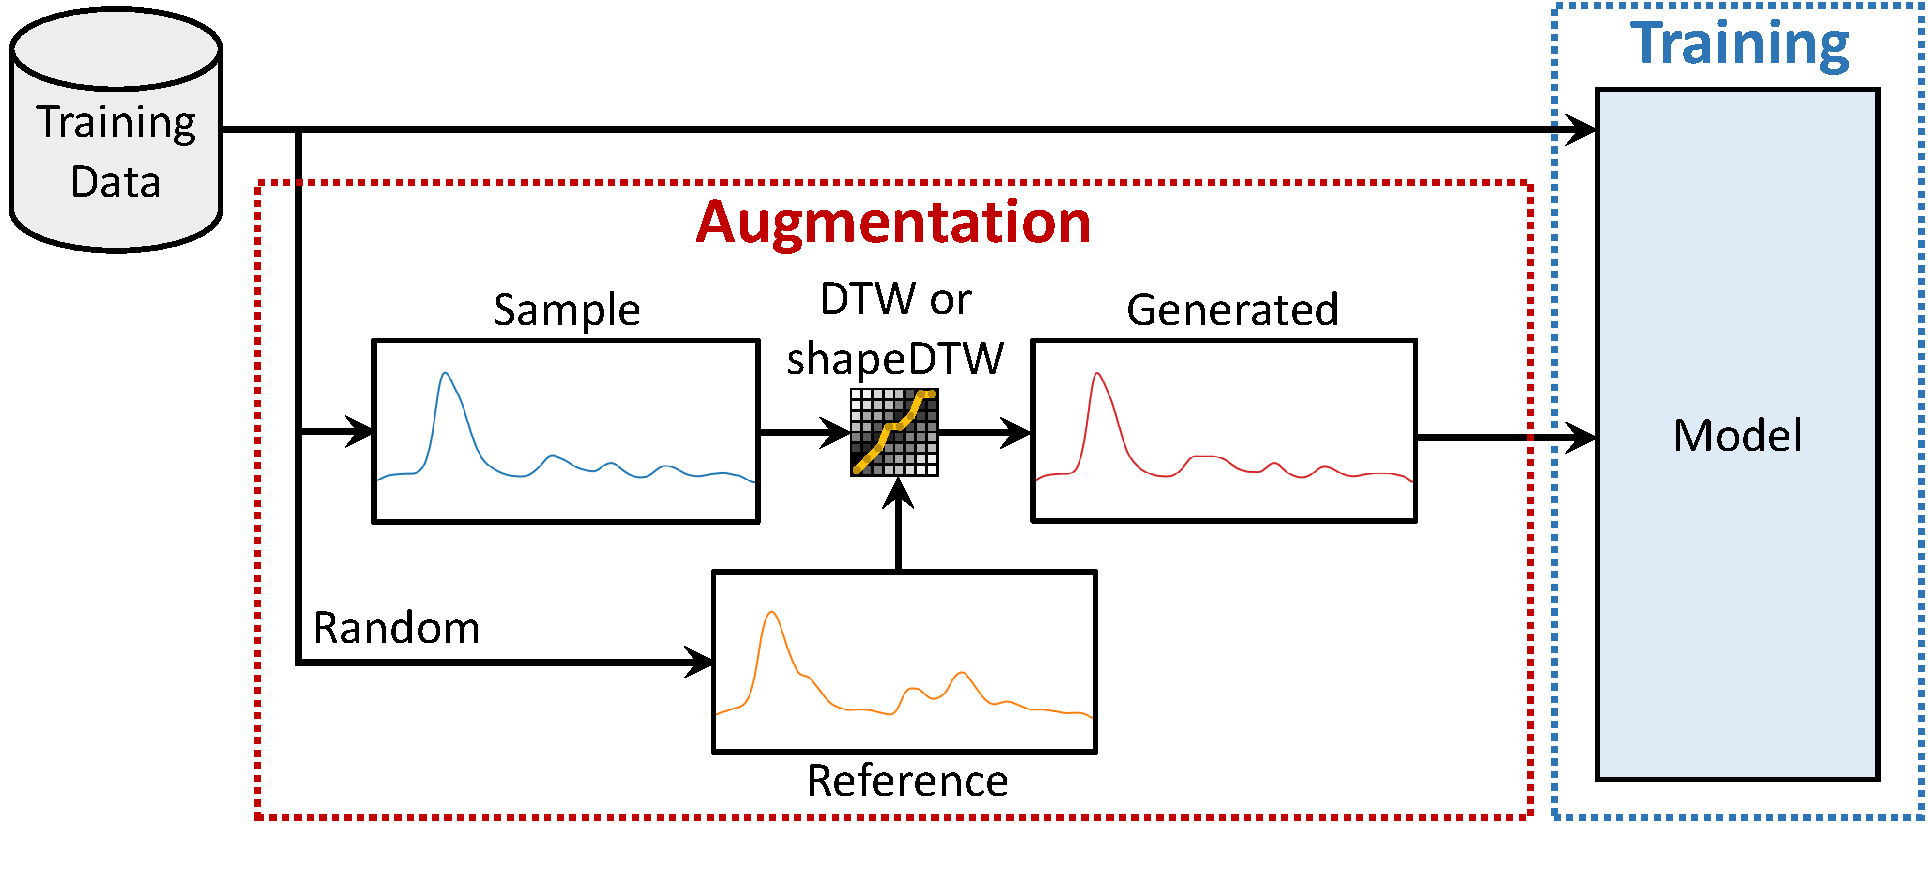
\includegraphics[page=1, width=0.9\textwidth]{./images/diagram_random.pdf}
\caption{Illustration of Random Guided Warping (RGW) and its variant using shapeDTW (RGWs)~\cite{iwana2020timeseriesdataaugmentation}. RGW aligns a time series with intra-class references using dynamic time warping (DTW), while RGWs leverages shapeDTW for enhanced alignment based on local shape descriptors~\cite{ZHAO2018171}.}
    \label{fig:rgw}
\end{figure}


Discriminative Guided Warping (DGW)~\cite{iwana2020timeseriesdataaugmentation} is similar to RGW, with the distinction that it uses multiple random (bootstrapped) subsets and directs from them for reference. The nearest centroid classifier utilizing DTW (or shapeDTW) distance determines the most discriminative directed reference from the bootstrapped sets. Rather than utilizing predictions from this classifier, a reference point with the largest distance between positive and negative centroids is selected. Utilizing this discriminatively selected reference, the temporal sequences are wrapped using  DTW or shapeDTW as previously described. Figure~\ref{fig:dgw} illustrates these techniques~\cite{iwana2020timeseriesdataaugmentation, 10.1371/journal.pone.0254841, ZHAO2018171}. In our experimental protocol, we utilize DGW for the DTW variant and DGWs for the shapeDTW variant.


\begin{figure}[h!]
    \centering
    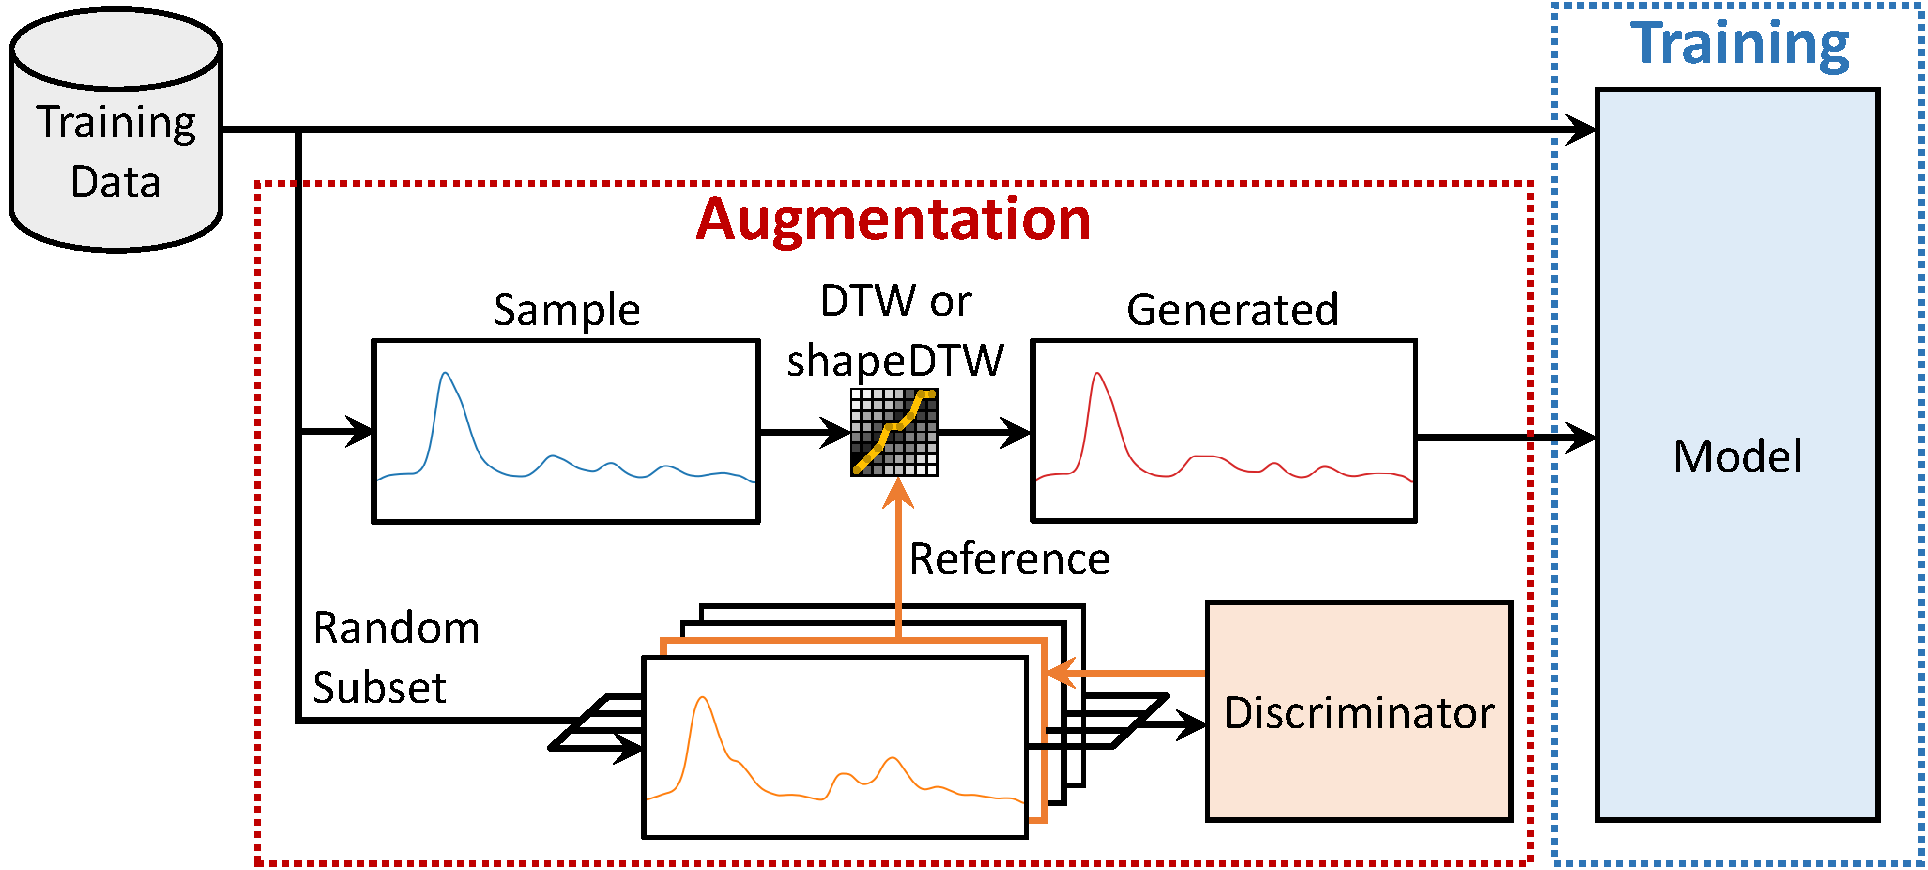
\includegraphics[page=1, width=0.9\textwidth]{./images/diagram_disc.pdf}
\caption{Illustration of the Discriminative Guided Warping (DGW) augmentation method~\cite{iwana2020timeseriesdataaugmentation}. DGW extends RGW by selecting a discriminative reference from bootstrapped intra-class subsets. The reference is chosen based on the largest centroid distance between classes using DTW or shapeDTW~\cite{ZHAO2018171}.}
    \label{fig:dgw}
\end{figure}




% new surveydi ela
\subsection{Generative Model-based Augmentations} \label{section:gan}



Deep generative models have become prominent in multiple fields, particularly image generation, due to their ability to produce realistic synthetic samples. Generative Adversarial Networks (GANs) are well-known among generative models for effectively generating diverse, realistic data that substantially improves training datasets. \cite{8512396} proposed a deep LSTM-based GAN for augmenting ECG and EEG signals. Subsequently, \cite{ramponi2019tcganconditionalgenerativeadversarial} introduced Temporal Convolutional GANs (TCGAN), which use one-dimensional convolutional layers to generate time series data. Conditional GANs (cGANs)~\cite{mirza2014conditionalgenerativeadversarialnets} have been utilized for data augmentation; however, \cite{9003933} compared a traditional GAN with a cGAN in the context of speech recognition and concluded that the traditional GAN exhibited better results on average~\cite{10.1371/journal.pone.0254841}. A recent generative model, TimeGAN, developed by \cite{timegan}, also expands these concepts to sequential data. Unlike traditional GANs, TimeGAN explicitly incorporates temporal dynamics, enabling the generation of highly realistic synthetic time series data~\cite{timegan}.



Figure~\ref{fig:timegan} outlines the architectural framework of TimeGAN, consisting of four primary components: an embedding function, a recovery function, a sequence generator, and a sequence discriminator. The embedding function transforms real sequences into a compacted latent space, while the recovery function reconstructs sequences from the latent representations. The generator creates latent representations of sequences, whereas the discriminator distinguishes between the latent embeddings of real and synthetic sequences. Unlike traditional GANs, TimeGAN optimizes unsupervised adversarial losses and supervised reconstruction losses, ensuring that the generated data is realistic and accurately represents the temporal dynamics of the original data~\cite{timegan}. 

\begin{figure}[h!]
    \centering
    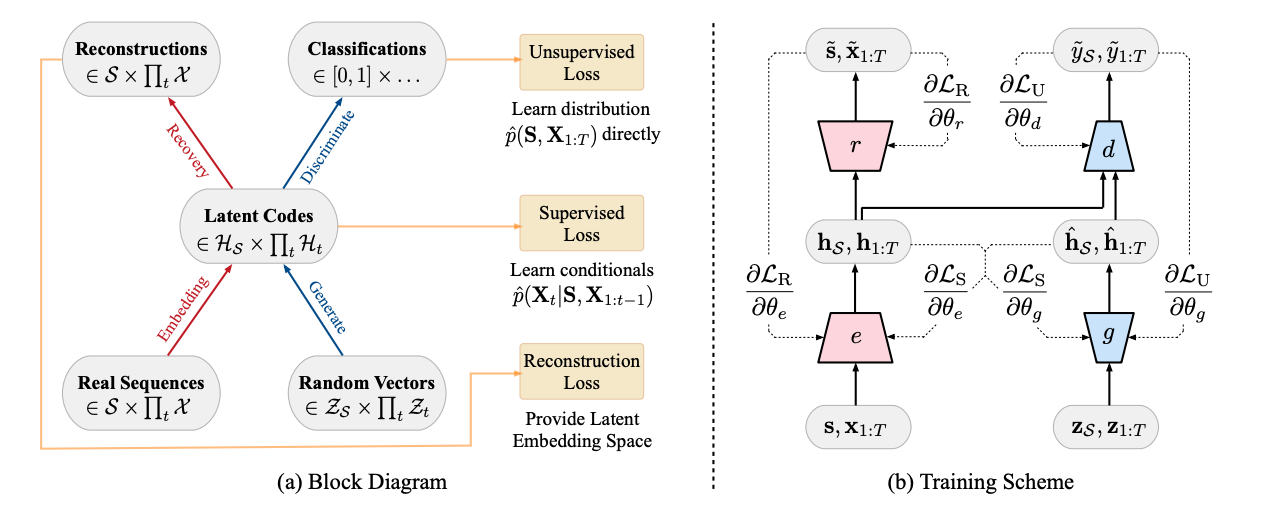
\includegraphics[page=1, width=0.9\textwidth]{./images/timegan.png}
\caption{TimeGAN architecture, consisting of an embedding function, recovery function, generator, and discriminator. The embedding-recovery pair maps time series to and from a latent space, while the generator and discriminator operate in this space to synthesize and evaluate sequences. TimeGAN combines adversarial and supervised losses to generate realistic time series that preserve temporal dynamics~\cite{timegan}.}

    \label{fig:timegan}
\end{figure}


In Section~\ref{section:other}, we mentioned that TimeGAN is removed from the experimentation protocol as it is computationally expensive, and other methods achieve better results for TSF. It is also true for TSC as the study~\cite{10.1371/journal.pone.0254841} has excluded it from the experimentations due to additional expensive external training. Other studies, such as \cite{gao2024dataaugmentationtimeseriesclassification} have shown that the GAN methods failed to generate realistic data (refer to Appendix~\ref{app:tscranking}), marking it the least effective augmentation, and \cite{10.1371/journal.pone.0315343} have indicated a marginal improvement over the baseline (see Table~\ref{tab:augmentation_performance}). These findings validated our decision to exclude them from our evaluations.







\subsection{Decomposition-based Augmentations}

Section~\ref{section:decom} discusses decomposition-based methods, which are primarily used for TSF. For TSC, similar approaches utilize techniques like EMD and STL to break down signals into independent or trend-related components. These components are then transformed or modified to generate augmented samples. The earlier methods using EMD (see Section~\ref{section:decom}) and MBB with STL (see Section~\ref{section:other}) are reviewed and discussed. Additionally, there are also augmentation methods that use RobustSTL~\cite{wen2018robuststlrobustseasonaltrenddecomposition} instead of other decompositions. However, unlike in forecasting, decomposition-based methods are excluded from our classification evaluations. Table~\ref{tab:augmentation_performance} shows that these methods underperform relative to the baseline and are the least effective augmentation techniques among 18 other methods. They have also been disregarded in other studies due to their limited effectiveness~\cite{nam2020data, 10.1371/journal.pone.0315343, 10.1371/journal.pone.0254841}.




\begin{table}[h!]
% increase table row spacing, adjust to taste
\renewcommand{\arraystretch}{1.3}
% if using array.sty, it might be a good idea to tweak the value of
% \extrarowheight as needed to properly center the text within the cells

\centering
% Some packages, such as MDW tools, offer better commands for making tables
% than the plain LaTeX2e tabular which is used here.
\scalebox{0.8}{
\begin{tabular}{c c c c r}
\hline
\textbf{Augmentation Methods} & \textbf{ResNet (\%)} & \textbf{Ranking}  \\
\hline
RGWs & 85.69 ± 15.12 & 1 \\
DGWs & 85.65 ± 15.19 & 2 \\
Window Warping & 85.55 ± 15.32 & 3 \\
Random Permutation & 85.44 ± 16.02 & 4 \\
SFCC & 85.43 ± 17.08 & 5 \\
DGW & 85.32 ± 15.28 & 6 \\
Permutation & 85.26 ± 16.58 & 7 \\
RGW & 85.21 ± 15.85 & 8 \\
DTW-Merge & 85.19 ± 15.67 & 9 \\
Window Slicing & 85.17 ± 15.62 & 10 \\
GAN & 85.15 ± 15.22 & 11 \\
\underline{None} & \underline{84.98 ± 16.41} & \underline{12} \\
wDBA & 84.78 ± 16.36 & 13 \\
Time Warping & 84.49 ± 15.39 & 14 \\
Scaling & 84.15 ± 17.27 & 15 \\
Jitter & 83.95 ± 17.52 & 16 \\
SPAWNER & 83.26 ± 17.07 & 17 \\
Magnitude Warping & 83.17 ± 17.75 & 18 \\
Rotation & 80.21 ± 19.93 & 19 \\
EMD & 76.57 ± 26.16 & 20 \\
\hline
\end{tabular}
}
\caption{Accuracy performance (\%) of various augmentation methods for time series classification (TSC) using ResNet, based on results reported in~\cite{gao2024dataaugmentationtimeseriesclassification}. Decomposition-based methods, such as EMD, perform the worst and fall behind the baseline (\underline{None}), confirming prior findings that they are less effective for TSC.}

\label{tab:augmentation_performance}
\end{table}